% Chapter 1

\chapter{\uppercase{Introduction}}
\label{Capitulo 1}

This document describes the development of a method for detecting anomalies in car driving. The use of Machine Learning techniques is proposed to generate a mechanism that identifies driving anomalies, so that they can be used to promptly alert agents and thus correct their driving behaviors.

%El presente documento describe el desarrollo de un m\'{e}todo para la detecci\'{o}n de anomal\'{i}as en la conducci\'{o}n de autom\'{o}viles. Se propone el uso de t\'{e}cnicas de Aprendizaje Autom\'{a}tico para generar un mecanismo que identifique anomal\'{i}as de manejo, de tal modo que \'{e}stas puedan usarse para alertar oportunamente a los agentes y as\'{i} logren correjir sus conductas de conducci\'{o}n.

\vspace{5mm} %5mm vertical space

The main idea is to generate a model that learns the normal driving behavior of a specific agent, to later autonomously detect those unexpected behaviors and report them as anomalies, so that a traffic accident can be avoided or the effects of it reduced.
%La idea principal, es generar un modelo que aprenda el comportamiento normal de conducci\'{o}n de un agente concreto, para posteriormente detectar de forma aut\'{o}noma aquellos comportamientos inesperados e informarlos como anomal\'{i}as, de manera que se pueda evitar  un accidente de tr\'{a}nsito o reducir los efectos del mismo.

\section{Approach of the problem}

Due to the serious consequences they cause on people and the high economic costs associated with them, traffic accidents are classified as a global social and public health problem.
%Debido a las graves secuelas que causan sobre las personas y los altos costos econ\'{o}micos asociados a ellos, los accidentes de tr\'{a}nsito se catalogan como un problema social y de salud p\'{u}blica mundial.

\vspace{5mm} %5mm vertical space

According to the World Health Organization (WHO) each year there are approximately 1.25 million deaths due to traffic accidents, adding that half of all these victims are pedestrians, cyclists and motorcyclists (See Figure \ref{fig:oms} page \pageref{fig:oms}). It can also be said that they are one of the most important causes of death in the world, and the main cause of death among people between the ages of 15 and 29.
%Seg\'{u}n la Organizaci\'{o}n Mundial de Salud (OMS) cada a\~{n}o existen aproximadamente 1,25 millones de muertes a causa de accidentes de tr\'{a}nsito, agregando que la mitad de todas estas victimas son peatones, ciclistas y motociclistas (V\'{e}ase la figura \ref{fig:oms} pag. \pageref{fig:oms}). Asimismo se puede decir que son una de las causas de muerte más importantes en el mundo, y la principal causa de muerte entre personas de edades comprendidas entre los 15 y los 29 años. 

\vspace{5mm} %5mm vertical space

\begin{figure}[h!]
  \begin{center}	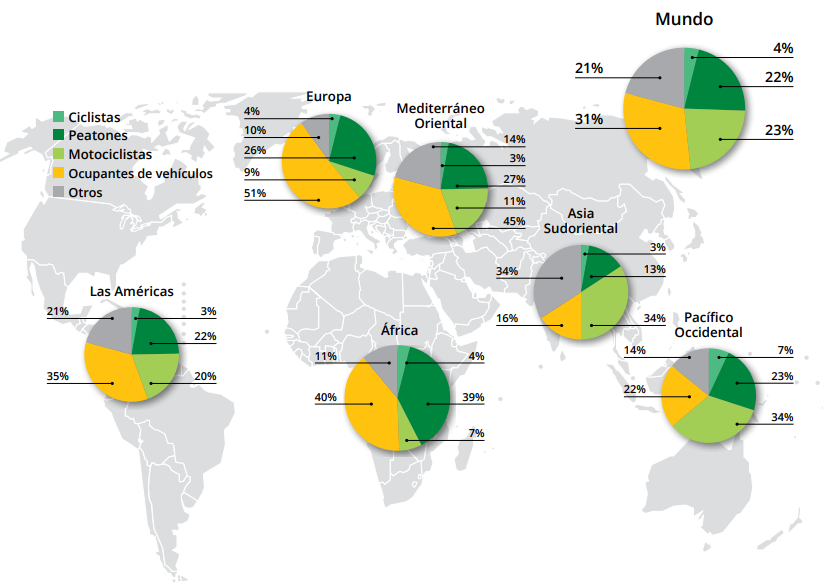
\includegraphics[width=0.9\textwidth, fbox]{imagenes/Cap1/oms1}
  \caption{Deaths due to traffic accidents by region depending on user's type \protect\cite{Reference65}.}
  \label{fig:oms}  
  \end{center}
\end{figure}

On the other hand, according to the Cochabamba Transit Operating Unit, the accidents recorded in 2017 caused the death of 200 people and left approximately 2200 injured.
%Por otro lado seg\'{u}n la Unidad Operativa de Tr\'{a}nsito de Cochabamba los accidentes registrados en 2017 provocaron la muerte de 200 personas y dejaron aproximadamente 2200 heridos.
	
\vspace{5mm} %5mm vertical space

Figure \ref{fig:arbol} shows the causes for which a traffic accident is caused, it can be seen that a large part of these are due to the human factor, however there are others that involve environmental and mechanical factors, so it is impossible completely avoid them.
%En la figura \ref{fig:arbol} se muestra las causas por las cuales se ocasiona un accidente de tr\'{a}nsito, se puede observar que gran parte de \'{e}stas se deben al factor humano sin embargo hay otras que conllevan factores medio-ambientales y mec\'{a}nicos, por lo que se hace imposible evitar completamente los mismos. 

\vspace{5mm} %5mm vertical space

That is why it is necessary to have mechanisms to prevent and/or act in a timely manner against possible traffic accidents, which is why this work focuses on studying driving behaviors, in order to generate alerts when finding a behavior anomalous in driving, so that the effects of it can be avoided or in any case minimized.
%Es por ello que se hace necesario el contar con mecanismos para prevenir y/o actuar de forma oportuna ante posibles accidentes de tr\'{a}nsito, motivo por el cual el presente trabajo se centra en estudiar los comportamientos de conducci\'{o}n, para as\'{i} generar alertas al encontrar un comportamiento an\'{o}malo en el manejo, de manera que se pueda evitar o en todo caso minimizar los efectos del mismo.

\begin{figure}[h!]
  \begin{center}	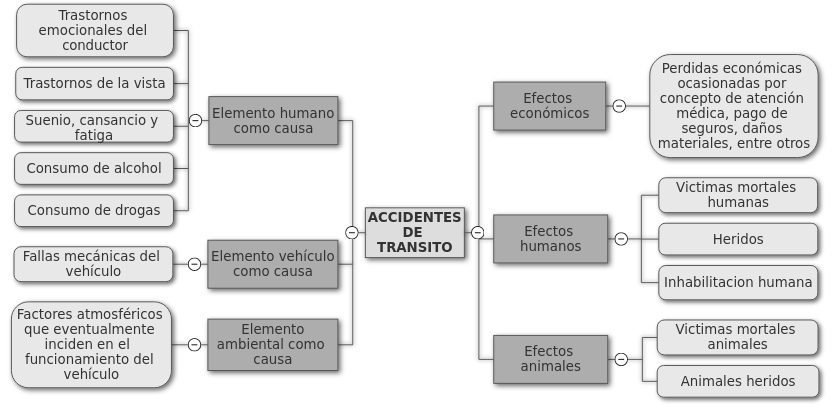
\includegraphics[width=1.0\textwidth, fbox]{imagenes/Cap1/arbol_p}
  \caption{Problem tree (Own elaboration).}
  \label{fig:arbol}
  \end{center}
\end{figure}


\section{General objective}

The general objective of the present work is to develop a mechanism for detecting driving anomalies, through the use of a mobile device and Machine Learning algorithms, in order to alert in a timely manner the finding of an anomalous driving pattern, such as tiredness, drunkenness, or health problems, eg. epilepsy.
%El objetivo general del presente trabajo es desarrollar un mecanismo de detecci\'{o}n de anomal\'{i}as de conducción, mediante el uso de un dispositivo móvil y algoritmos de Aprendizaje Automático, con el fin de alertar de forma oportuna el hallazgo de un patrón anómalo en el manejo, tal como cansancio, ebriedad, o problemas de salud, ej, epilepsia.

\section{Specific objectives}
\begin{itemize}
\item Capture the driving parameters of a driver by using sensors of a mobile device.
\item Scale parameters using data pre-processing techniques.
\item Generate a Machine Learning model that adjusts to normal driving behavior.
\item Define an anomaly detection method to generate an abnormal driving alert.
\item Evaluate the anomaly detection method with new samples

%\item Capturar los parámetros de manejo de un conductor mediante el uso de sensores de un dispositivo móvil.
%\item Escalar los parámetros de manejo mediante técnicas de pre-procesamiento de datos.
%\item Generar un modelo de aprendizaje automático que se ajuste a un comportamiento normal de manejo.
%\item Definir un método de detección de anomalías para generar una alerta de conducción anormal.
%\item Evaluar el método de detección de anomalías con nuevas muestras.

\end{itemize}

\section{Justification}

Traffic accidents charge an unacceptable number of victims each year, especially in the poorest regions of the world. This is due to various aspects, but the main one lies in the low level of citizen awareness that exists, which leads to many people driving under the influence of alcohol, with excessive speed, manipulating their mobile devices, among others. For this reason, this work seeks to establish patterns of driving behaviors through the use of a mobile device and Machine Learning techniques, so that it is possible to detect timely driving anomalies.
%Los accidentes de tránsito cobran un número inaceptable de víctimas cada a\~{n}o, especialmente en las regiones m\'{a}s pobres del mundo. Esto se debe a diversos aspectos, pero el principal recae en el bajo nivel de conciencia ciudadana que existe, lo que conlleva a que muchas personas conduzcan bajo los efectos del alcohol, con exceso de velocidad, manipulando sus dispositivos m\'{o}viles, entre otros. Por ello este trabajo busca establecer patrones de comportamientos de conducci\'{o}n mediante el uso de un dispositivo m\'{o}vil y t\'{e}cnicas de Aprendizaje Autom\'{a}tico, de manera que se logre realizar una detecci\'{o}n de anomal\'{i}as de conducci\'{o}n oportuna.

\subsection{Practical justification}

Detect driving anomalies allows the authorities or agents to generate a timely alert so that they can correct their driving behaviors quickly. This way we can avoid traffic accidents or minimize their effects, thus reducing the amount of damage, both material and personal.
%Detectar anomal\'{i}as de conducci\'{o}n permite generar una alerta oportuna a las autoridades o a los agentes para que logren corregir sus conductas de conducci\'{o}n de forma r\'{a}pida. De esta manera se podr\'{a} evitar accidentes de tr\'{a}nsito o minimizar sus efectos, permitiendo as\'{i} reducir la cantidad de da\~{n}os, tanto materiales como personales.

\subsection{Methodological justification}

The study carried out in the development of this research allows highlighting the efficiency of Artificial Intelligence techniques in  detection of anomalies.
%El estudio realizado en el desarrollo del presente trabajo de investigaci\'{o}n permite resaltar la eficiencia de las t\'{e}cnicas de Inteligencia Artificial en la detecci\'{o}n de anomal\'{i}as.

\section{Limits and scope}

Due conducting field tests for this investigation is quite dangerous, the examples of anomalous driving were limited to:
%Debido a que la realizaci\'{o}n de pruebas de campo para \'{e}sta investigaci\'{o}n es bastante peligrosa, se limit\'{o} los ejemplos de conducci\'{o}n an\'{o}mala a:
\begin{itemize}
\item Dry brakes.
\item Turn right and left at high speed.
\item Turn abrupt zig zag.
\end{itemize}

\vspace{5mm} %5mm vertical space

Thus, experiments and tests were performed only on a small set of anomalous samples, therefore it is not expected that the proposed detection model will work correctly on those examples that were not considered.
%Siendo as\'{i}, los experimentos y pruebas se realizaron s\'{o}lo sobre un peque\~{n}o conjunto de ejemplos an\'{o}malos, por lo tanto no se espera que el modelo de detecci\'{o}n propuesto funcione de manera correcta sobre aquellos ejemplos que no fueron considerados.

\section{Research method}

The present study was conducted with an experimental approach, with the following hypothesis:
%El presente estudio se realiz\'{o} con un enfoque experimental, teniendo como hip\'{o}tesis la siguiente:


\begin{center}
\textit{\large{Is it possible to detect driving anomalies by using a mobile device and Machine Learning algorithms?}}
\end{center}

